\chapter{Support Vector Machines (SVM) - Experiments}

\par SVM has been widely used in text based detection techniques~\cite{1}. In this section we will analyze how SVM can be used in image spam detection. SVM is a supervised classification algorithm. SVM generates a separating hyper-plane at the end of the training phase which separates our data into two classes~\cite{8}. 



\section{Experiments}
\par Fig. \ref{fig:svm_detection_model}. shows the flow of train and test phases for the SVM Detection Model. First the ham and spam data is split into train and test sets. Train and test sets are exclusive i.e. there is no overlap between the two. 41 features are then extracted from the datasets. We then train the SVM Classifier with scaled train data. Test set is then passed to the SVM Classifier for detection. Additionally, in the train phase, feature selector is added to perform dimensionality reduction based on feature weights. 

\begin{figure}[h]
	\centering
	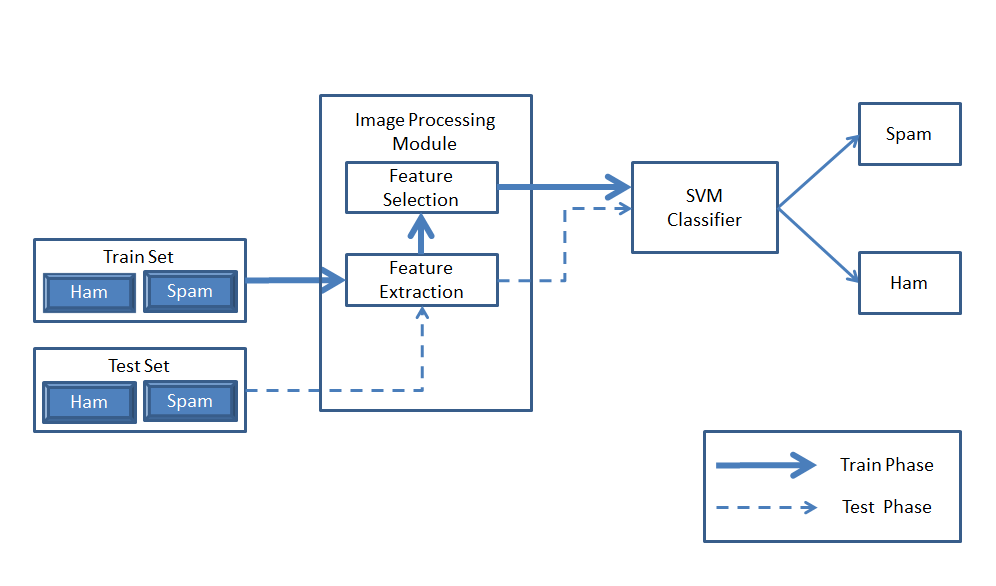
\includegraphics[width=.9\textwidth]{images/svm-flow.PNG}
	\caption{SVM Detection Model}
	\label{fig:svm_detection_model}
\end{figure}

\par To analyze the weight of each feature we calculated SVM scores for each feature individually. Fig. \ref{fig:AUC_individualFeatures}. shows SVM scores for individual features for all the three datasets. It is easy to note from the three graphs that the SVM AUC scores for individual features for test dataset has gone down significantly compared to those of Dataset 1 and 2.

\begin{figure}[h]	
	\begin{subfigure}{\textwidth}
		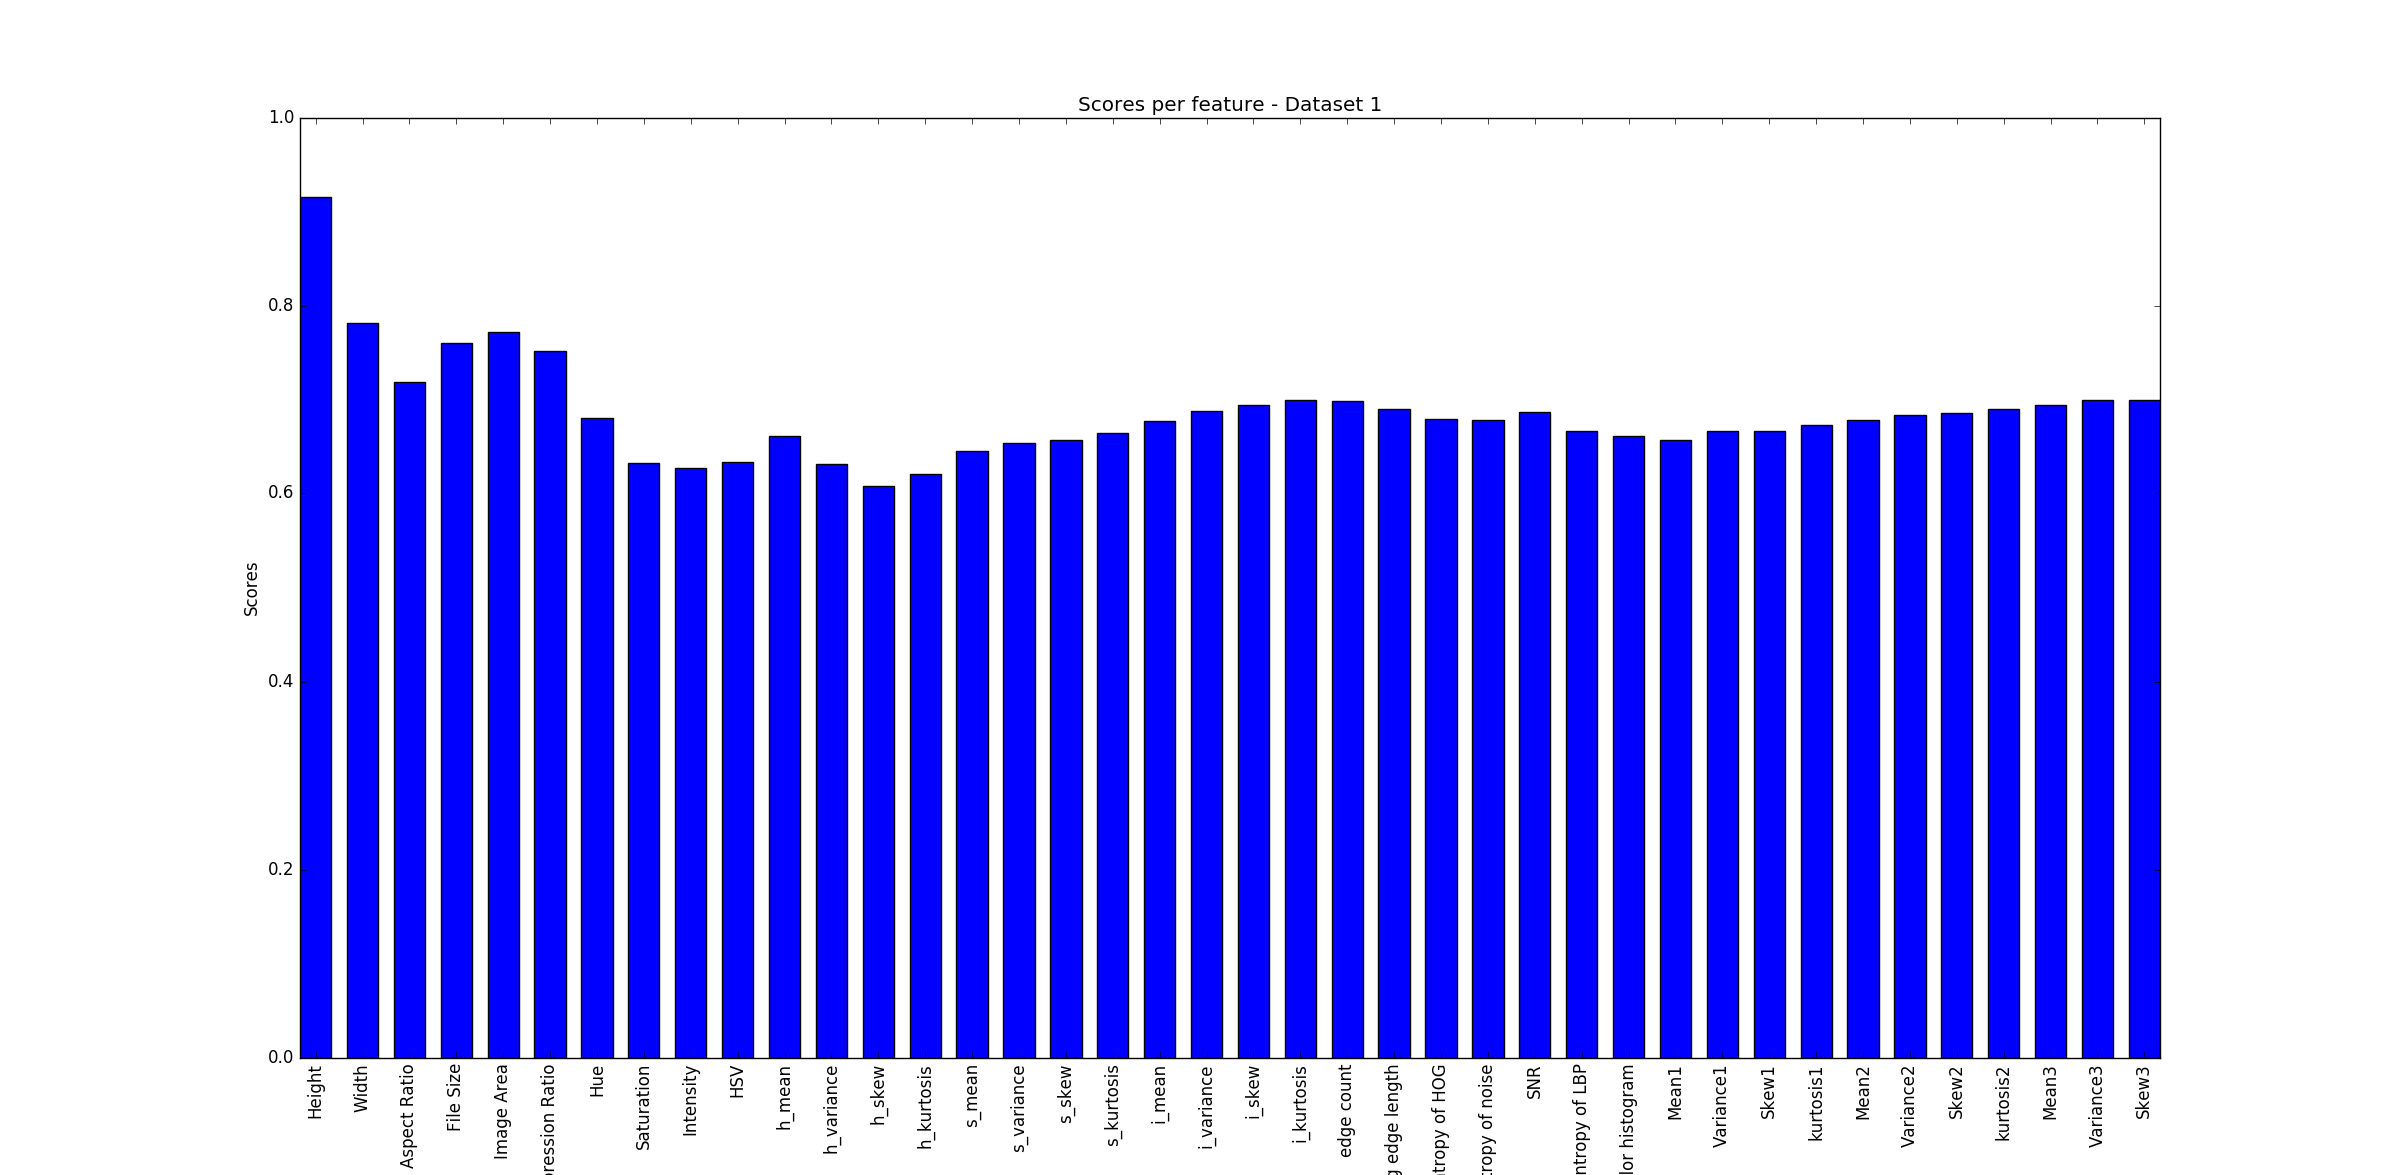
\includegraphics[width=\textwidth]{images/Dataset1-SVM-IndividualFeatures} 
		\caption{Dataset 1 AUC scores for Individual Features}
		\label{fig:AUC_Dataset1_individualFeature}
	\end{subfigure}
	\begin{subfigure}{\textwidth}
		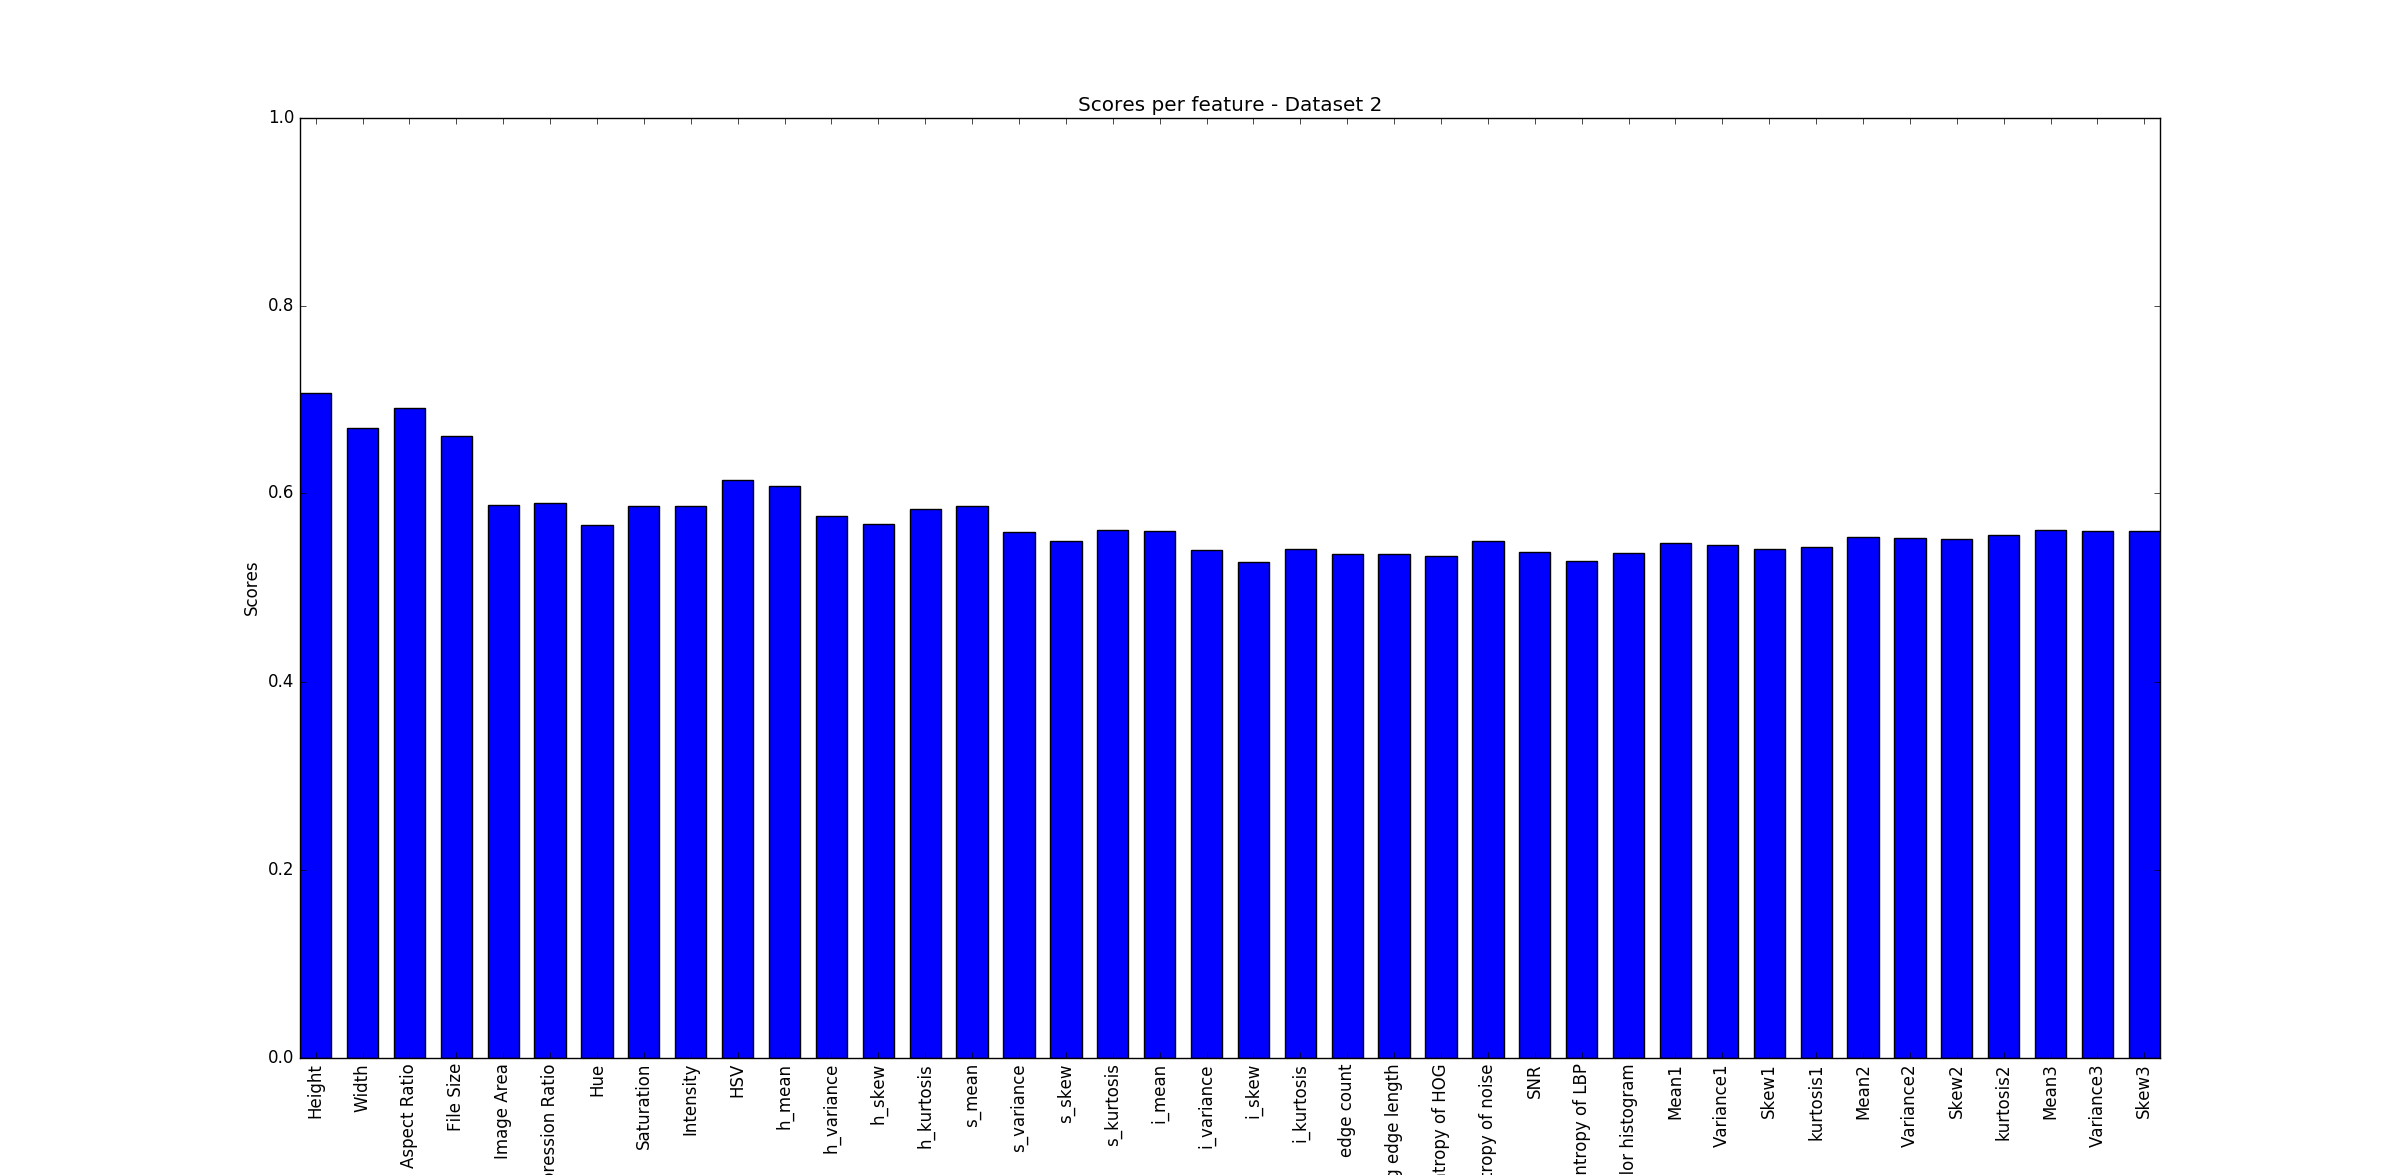
\includegraphics[width=\textwidth]{images/Dataset2-SVM-IndividualFeatures}
		\caption{Dataset 2 AUC scores for Individual Features}
		\label{fig:AUC_Dataset2_individualFeature}
	\end{subfigure}
	
	\begin{subfigure}{\textwidth}
		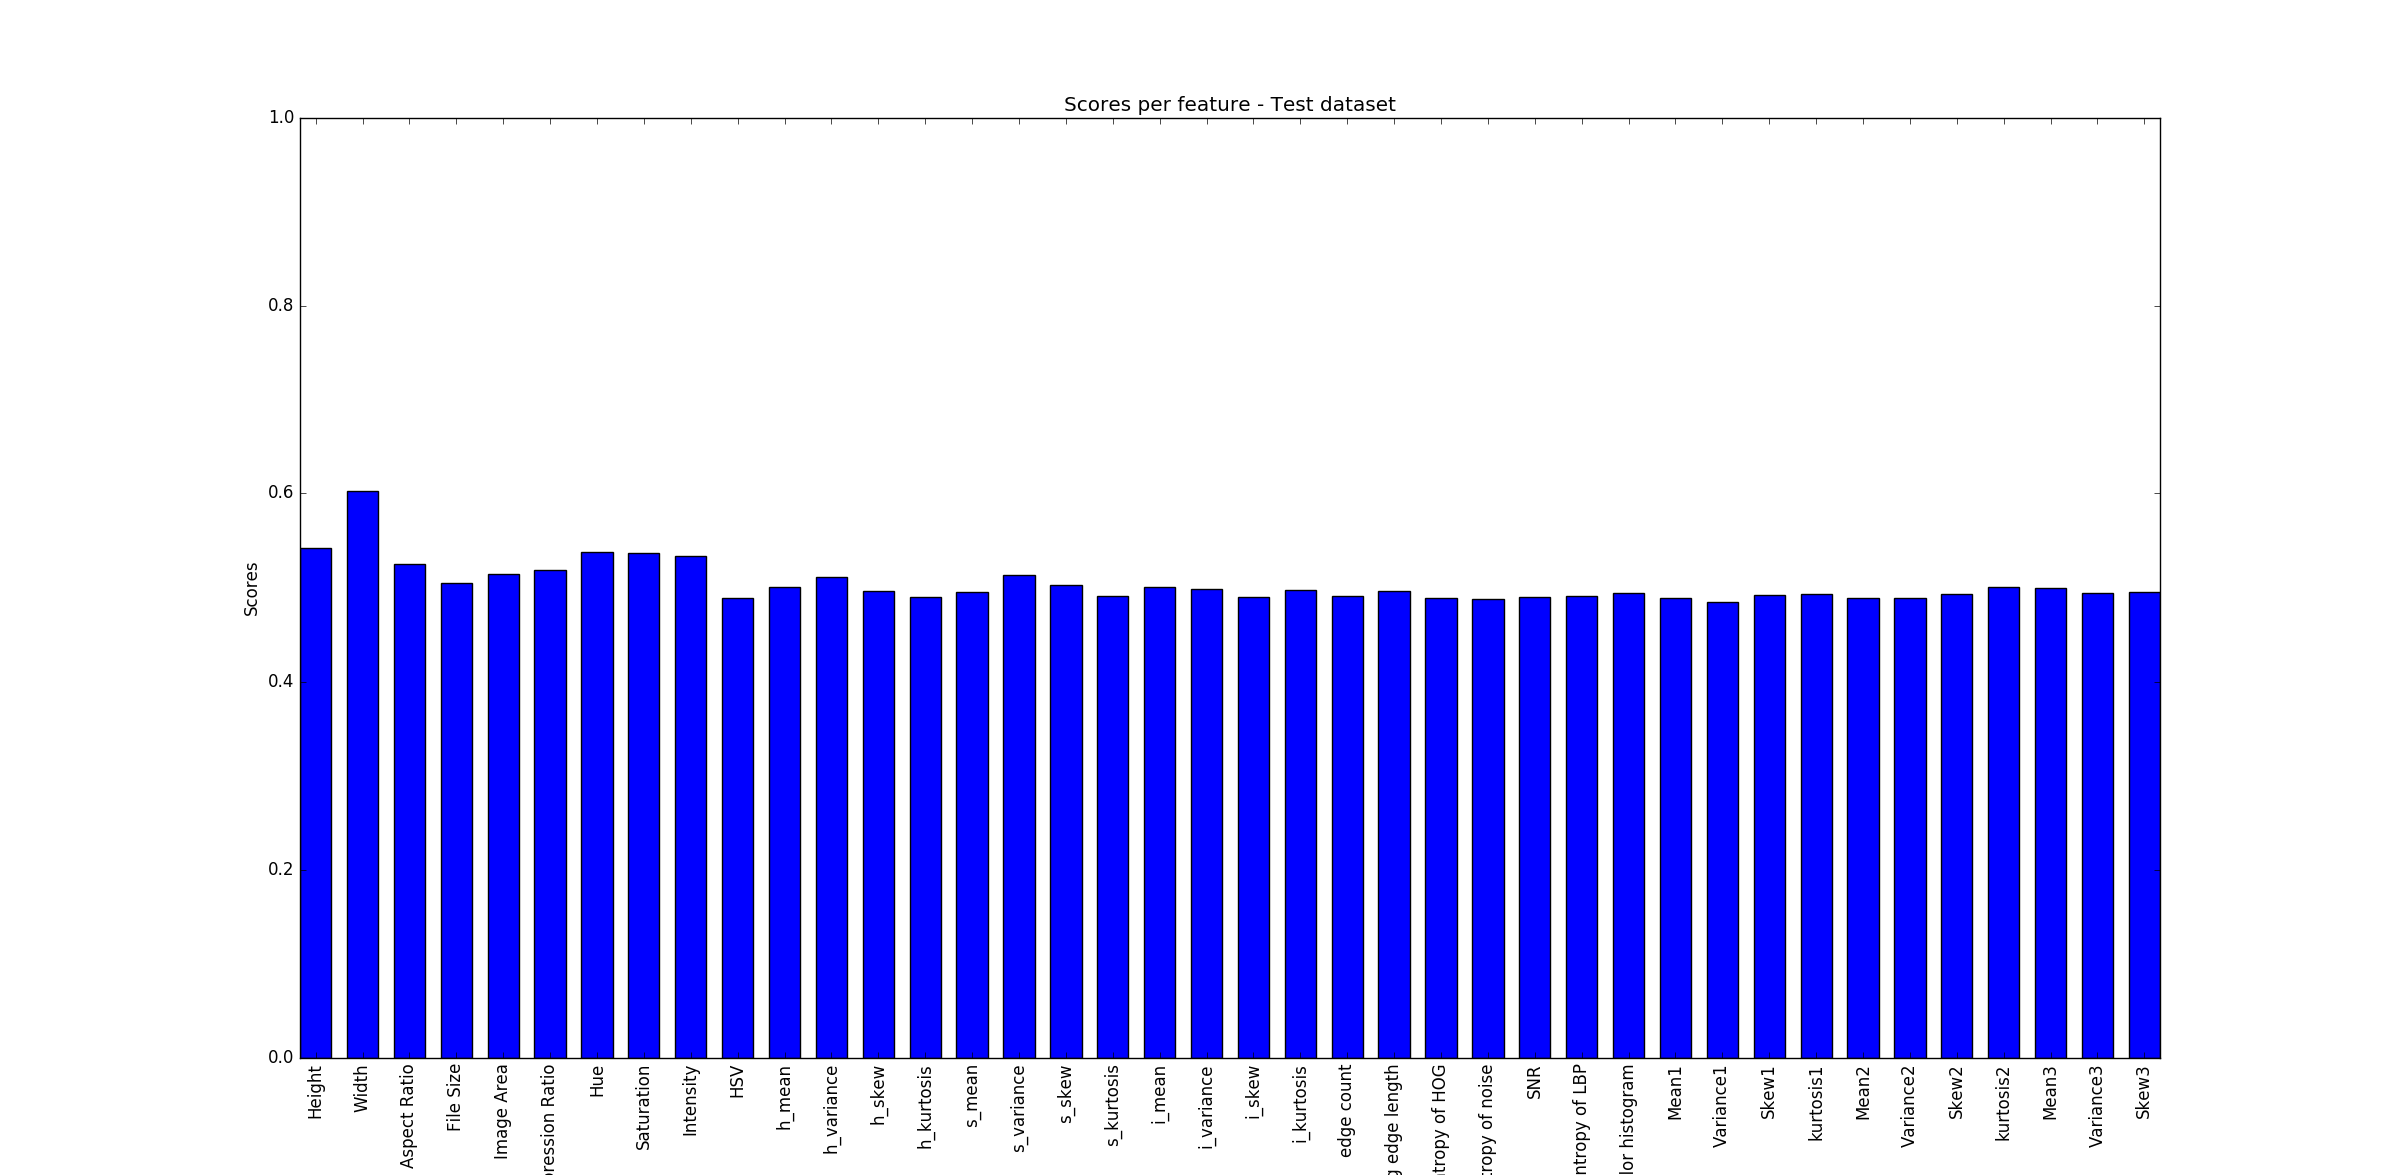
\includegraphics[width=\textwidth]{images/TestDataset-SVM-IndividualFeatures}
		\caption{Test Dataset AUC scores for Individual Features}
		\label{fig:AUC_Dataset3_individualFeature}
	\end{subfigure}
	
	\caption{AUC for individual features}
	\label{fig:AUC_individualFeatures}
\end{figure}


\subsection{Dataset 1}
\par All 41 features were extracted and scaled for dataset 1. We used 6\% of ham and spam images as training set and rest for testing. A total of 55 spam and 48 ham images were used as train objects. Remaining 865 spam images and 762 ham images were used for testing. Table \ref{table:dataset1_svm_results} shows the accuracies and False Positive Rates for each of the three SVM Kernels. We achieved best results for Linear Kernel. Fig. \ref{fig:Dataset1_linear_results}. shows the ROC curve and confusion matrix for linear kernel.

\begin{table}[htb]
	\centering
		\caption{Dataset 1 - SVM Results}
		\begin{tabular}{ |c|c|c| } 
			\hline
			Kernel & Accuracy & FPR \\
			\hline
			Linear & 0.97 & 0.06 \\ 
			\hline
			RBF & 0.96 & 0.07 \\ 
			\hline
			Poly & 0.95 & 0.08 \\ 
			\hline
		\end{tabular}
	\label{table:dataset1_svm_results}
\end{table}



\begin{figure}[h]
	
	\begin{subfigure}{0.5\textwidth}
		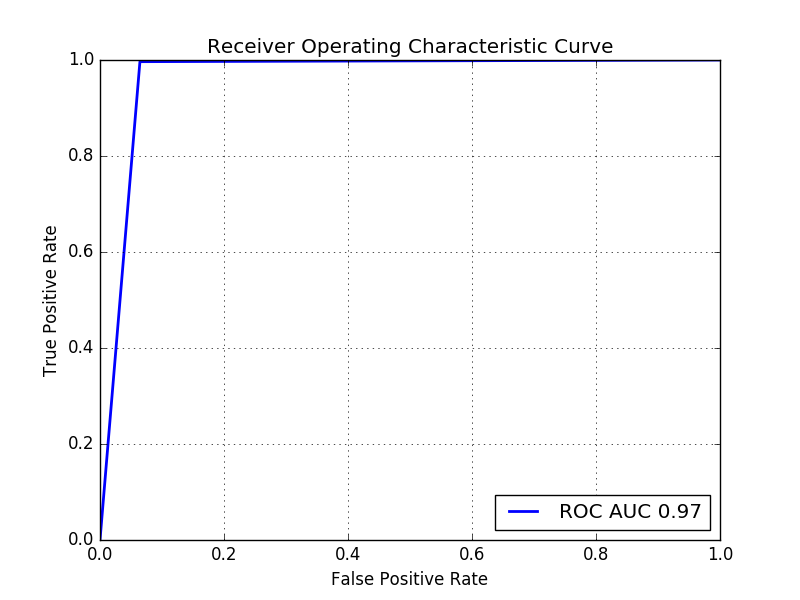
\includegraphics[width=0.9\linewidth]{images/AUC-Dataset1-linear} 
		\caption{ROC Curve}
		\label{fig:AUC_Dataset1_linear}
	\end{subfigure}
	\begin{subfigure}{0.5\textwidth}
		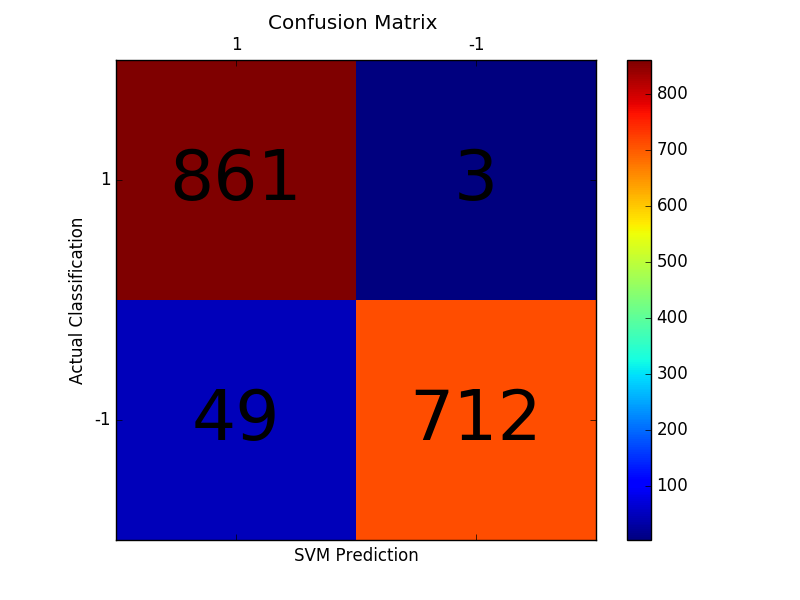
\includegraphics[width=0.9\linewidth]{images/CM-Dataset1-linear}
		\caption{Confusion Matrix}
		\label{fig:CM_Dataset1_linear}
	\end{subfigure}
	
	\caption{Dataset 1 - Linear Kernel}
	\label{fig:Dataset1_linear_results}
\end{figure}



\begin{figure}[h]
	
	\begin{subfigure}{0.5\textwidth}
		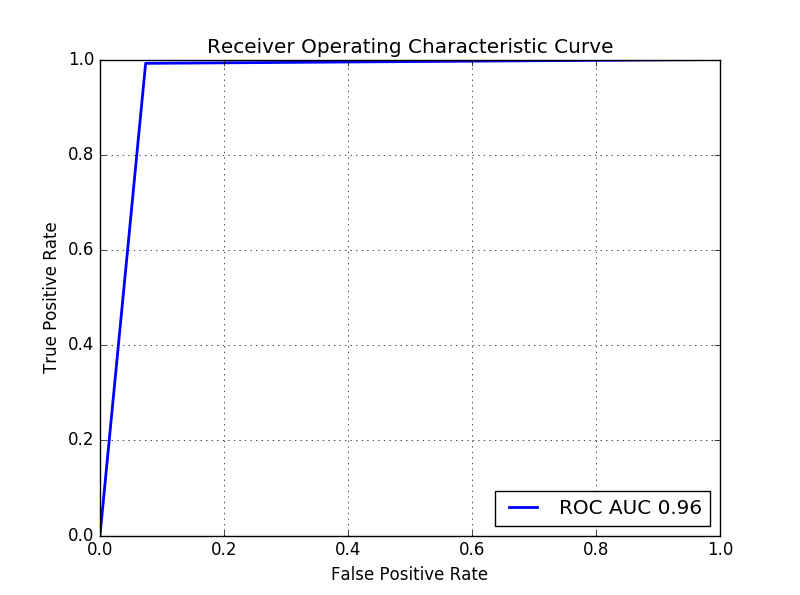
\includegraphics[width=0.9\linewidth]{images/AUC-Dataset1-rbf} 
		\caption{ROC Curve}
		\label{fig:AUC_Dataset1_rbf}
	\end{subfigure}
	\begin{subfigure}{0.5\textwidth}
		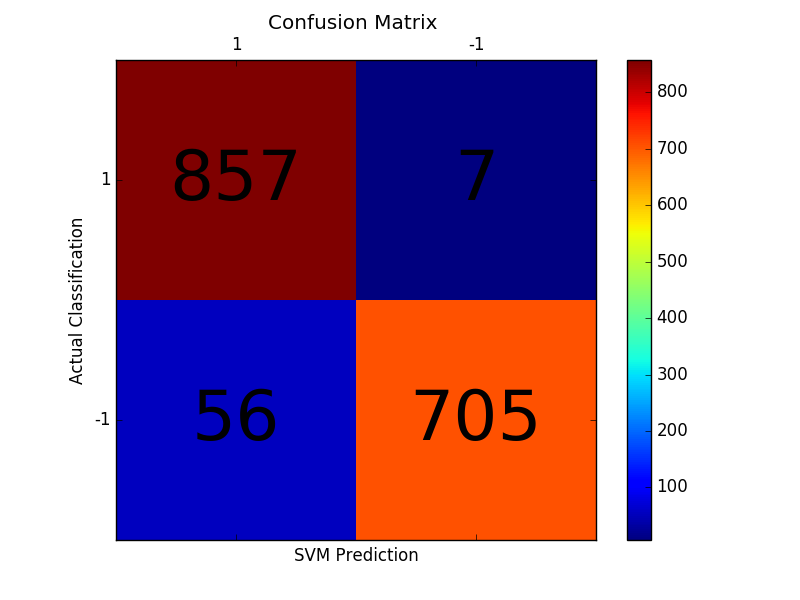
\includegraphics[width=0.9\linewidth]{images/CM-Dataset1-rbf}
		\caption{Confusion Matrix}
		\label{fig:CM_Dataset1_rbf}
	\end{subfigure}
	
	\caption{Dataset 1 - RBF Kernel}
	\label{fig:Dataset1_rbf_results}
\end{figure}


\begin{figure}[h]
	
	\begin{subfigure}{0.5\textwidth}
		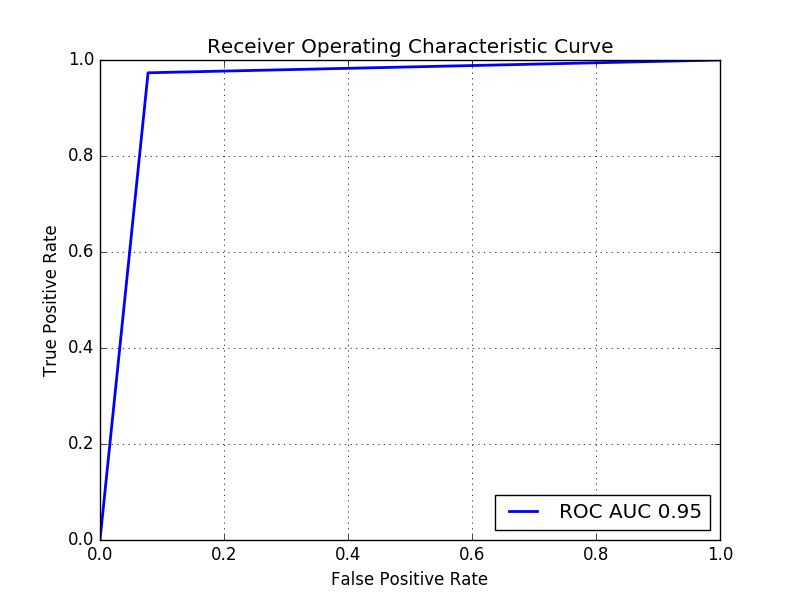
\includegraphics[width=0.9\linewidth]{images/AUC-Dataset1-poly} 
		\caption{ROC Curve}
		\label{fig:AUC_Dataset1_poly}
	\end{subfigure}
	\begin{subfigure}{0.5\textwidth}
		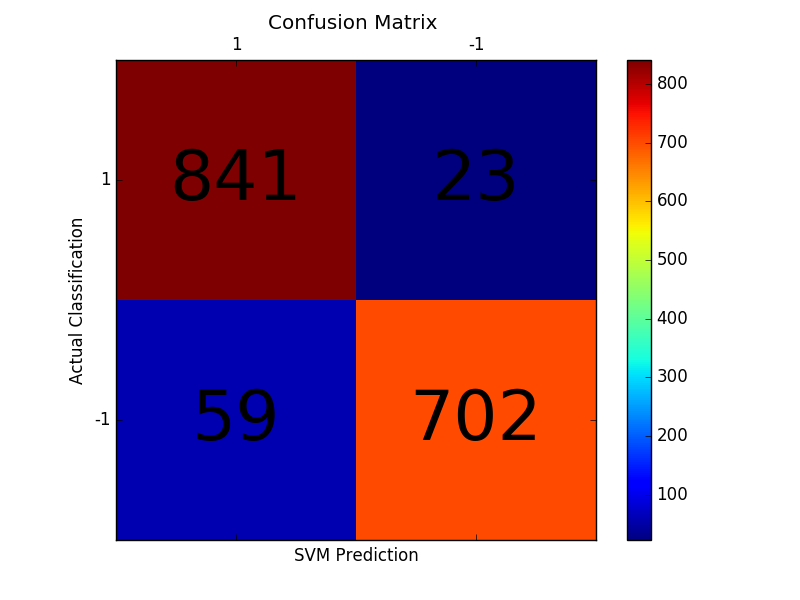
\includegraphics[width=0.9\linewidth]{images/CM-Dataset1-poly}
		\caption{Confusion Matrix}
		\label{fig:CM_Dataset1_poly}
	\end{subfigure}
	
	\caption{Dataset 1 - Polynomial Kernel}
	\label{fig:Dataset1_poly_results}
\end{figure}




\subsection{Dataset 2}
\par All 41 features were extracted and scaled for our in-house generated test dataset. We used 45\% of ham and spam images as training set and rest for testing. A total of 490 spam and 463 ham images were used as train objects. Remaining 599 spam images and 566 ham images were used for testing. Table \ref{table:Dataset2_svm_results} shows the accuracies and False Positive Rates for each of the three SVM Kernels. We achieved similar results for Linear and rbf kernels.


\begin{table}[htb]
	\centering
	\caption{Dataset 2 - SVM Results}
	\begin{tabular}{ |c|c|c| } 
		\hline
		Kernel & Accuracy & FPR \\
		\hline
		Linear & 0.98 & 0.02 \\ 
		\hline
		RBF & 0.98 & 0.02 \\ 
		\hline
		Poly & 0.95 & 0.10 \\ 
		\hline
	\end{tabular}
	\label{table:Dataset2_svm_results}
\end{table}



\begin{figure}[h]
	
	\begin{subfigure}{0.5\textwidth}
		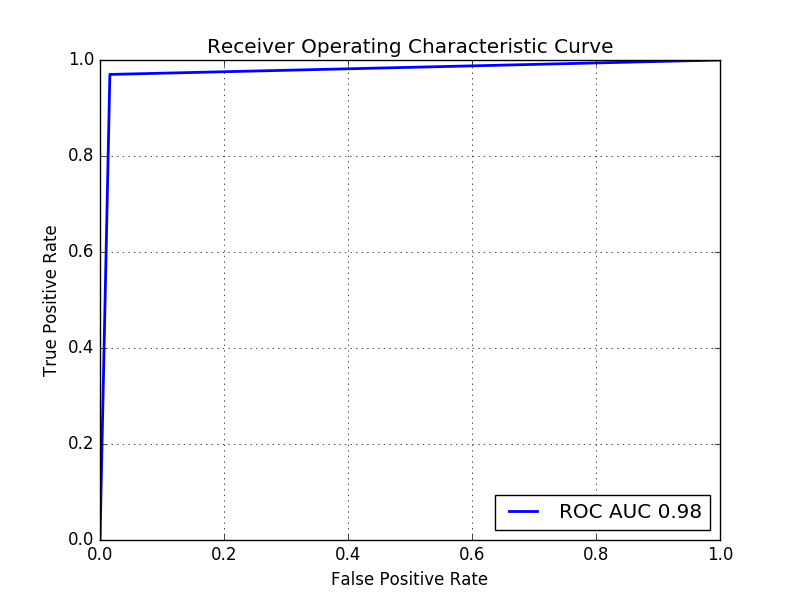
\includegraphics[width=0.9\linewidth]{images/AUC-Dataset2-linear} 
		\caption{ROC Curve}
		\label{fig:AUC_Dataset2_linear}
	\end{subfigure}
	\begin{subfigure}{0.5\textwidth}
		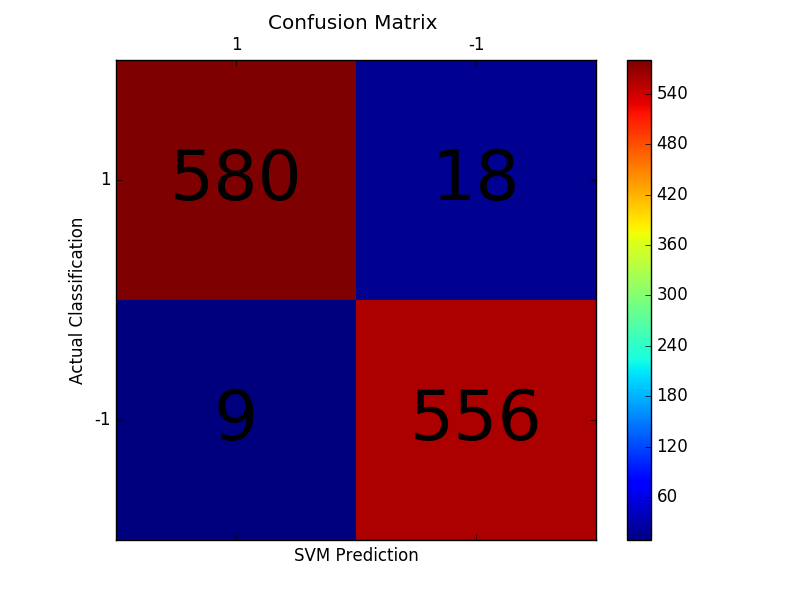
\includegraphics[width=0.9\linewidth]{images/CM-Dataset2-linear}
		\caption{Confusion Matrix}
		\label{fig:CM_Dataset2_linear}
	\end{subfigure}
	
	\caption{Dataset 2 - Linear Kernel}
	\label{fig:Dataset2_linear_results}
\end{figure}



\begin{figure}[h]
	
	\begin{subfigure}{0.5\textwidth}
		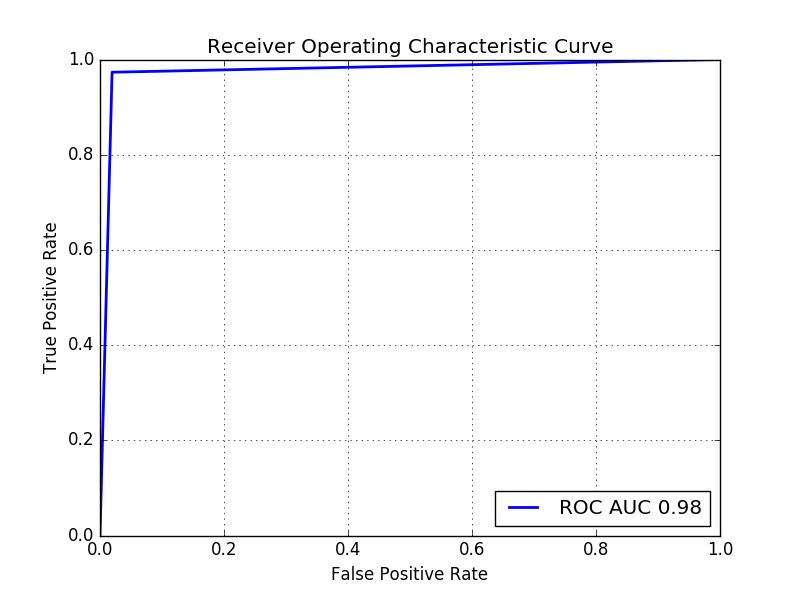
\includegraphics[width=0.9\linewidth]{images/AUC-Dataset2-rbf} 
		\caption{ROC Curve}
		\label{fig:AUC_Dataset2_rbf}
	\end{subfigure}
	\begin{subfigure}{0.5\textwidth}
		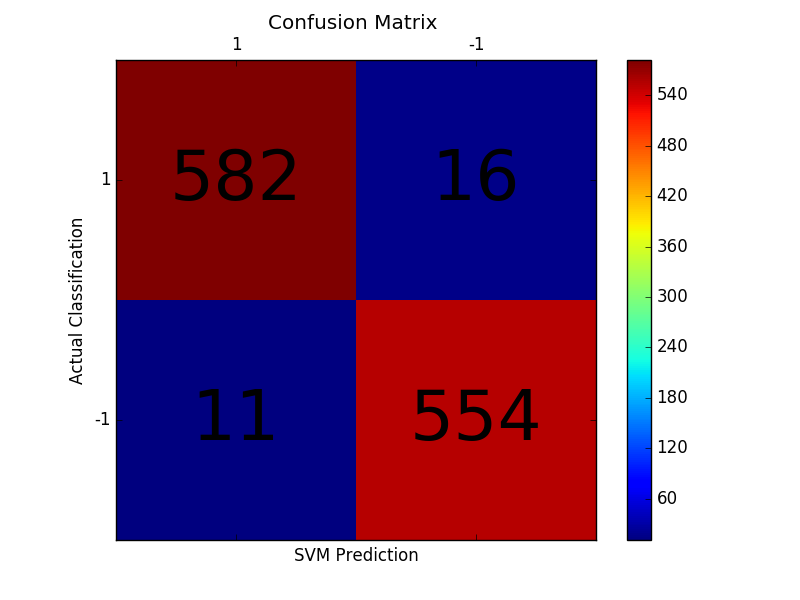
\includegraphics[width=0.9\linewidth]{images/CM-Dataset2-rbf}
		\caption{Confusion Matrix}
		\label{fig:CM_Dataset2_rbf}
	\end{subfigure}
	
	\caption{Dataset 2 - RBF Kernel}
	\label{fig:Dataset2_rbf_results}
\end{figure}


\begin{figure}[h]
	
	\begin{subfigure}{0.5\textwidth}
		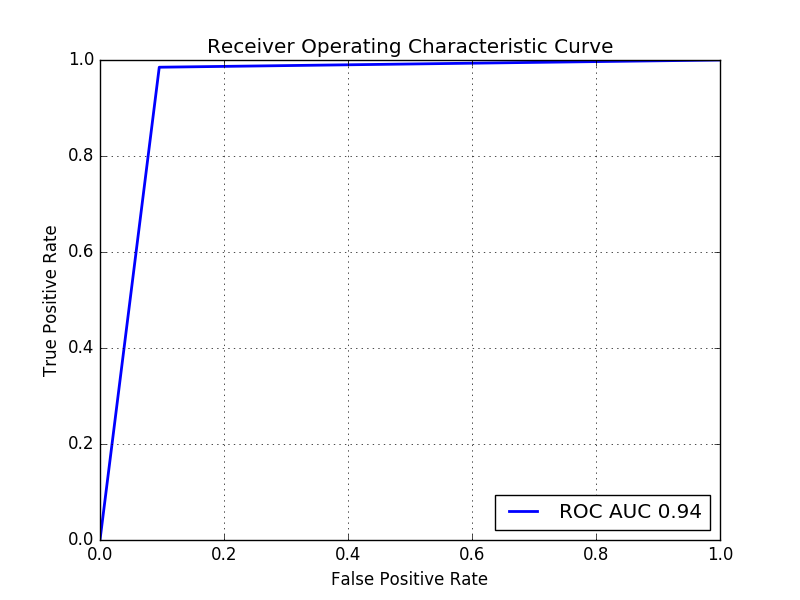
\includegraphics[width=0.9\linewidth]{images/AUC-Dataset2-poly} 
		\caption{ROC Curve}
		\label{fig:AUC_Dataset2_poly}
	\end{subfigure}
	\begin{subfigure}{0.5\textwidth}
		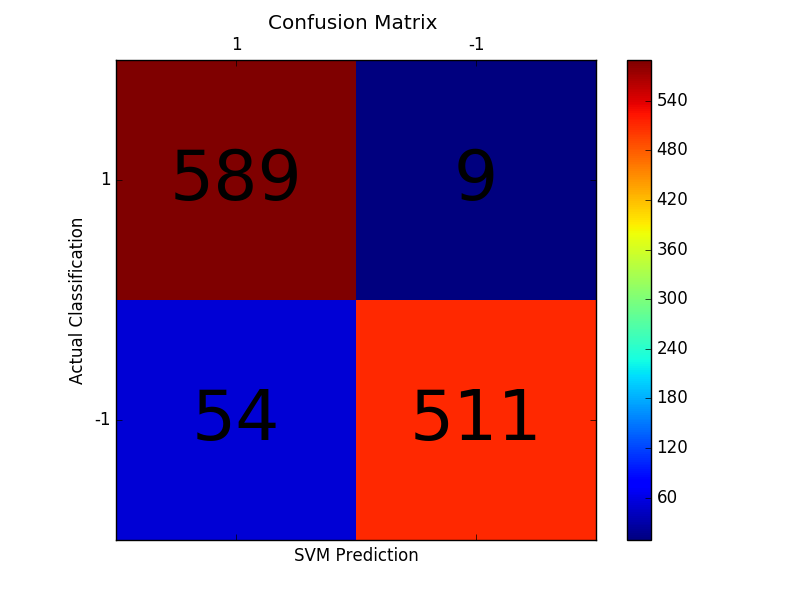
\includegraphics[width=0.9\linewidth]{images/CM-Dataset2-poly}
		\caption{Confusion Matrix}
		\label{fig:CM_Dataset2_poly}
	\end{subfigure}
	
	\caption{Dataset 2 - Polynomial Kernel}
	\label{fig:Dataset2_poly_results}
\end{figure}




\subsection{Dataset 3}
\par All 41 features were extracted and scaled for our in-house generated test dataset. We used 30\% of ham and spam images as training set and rest for testing. A total of 243 spam and 243 ham images were used as train objects. Remaining 567 spam images and 567 ham images were used for testing. Table \ref{table:testDataset_svm_results} shows the accuracies and False Positive Rates for each of the three SVM Kernels. We achieved best results for Linear Kernel.

\begin{table}[htb]
	\centering
	\caption{Test Dataset - SVM Results}
	\begin{tabular}{ |c|c|c| } 
		\hline
		Kernel & Accuracy & FPR \\
		\hline
		Linear & 0.70 & 0.38 \\ 
		\hline
		RBF & 0.64 & 0.34 \\ 
		\hline
		Poly & 0.56 & 0.78 \\ 
		\hline
	\end{tabular}
	\label{table:testDataset_svm_results}
\end{table}



\begin{figure}[h]
	
	\begin{subfigure}{0.5\textwidth}
		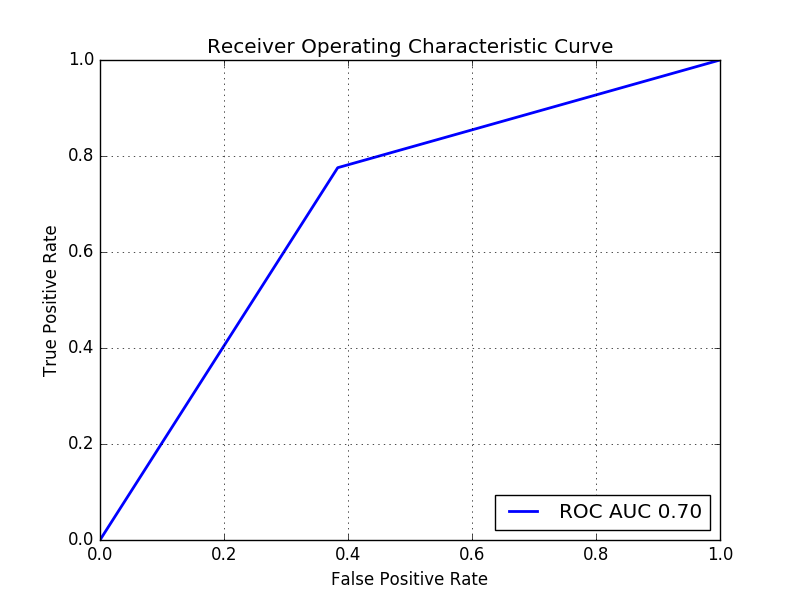
\includegraphics[width=0.9\linewidth]{images/AUC-TestDataset-linear} 
		\caption{ROC Curve}
		\label{fig:AUC_TestDataset_linear}
	\end{subfigure}
	\begin{subfigure}{0.5\textwidth}
		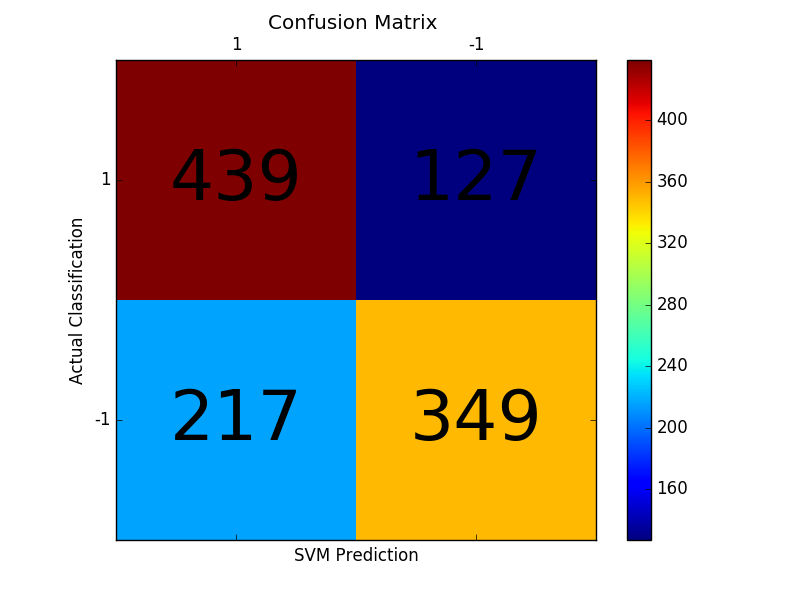
\includegraphics[width=0.9\linewidth]{images/CM-TestDataset-linear}
		\caption{Confusion Matrix}
		\label{fig:CM_TestDataset_linear}
	\end{subfigure}
	
	\caption{Test Dataset - Linear Kernel}
	\label{fig:TestDataset_linear_results}
\end{figure}



\begin{figure}[h]
	
	\begin{subfigure}{0.5\textwidth}
		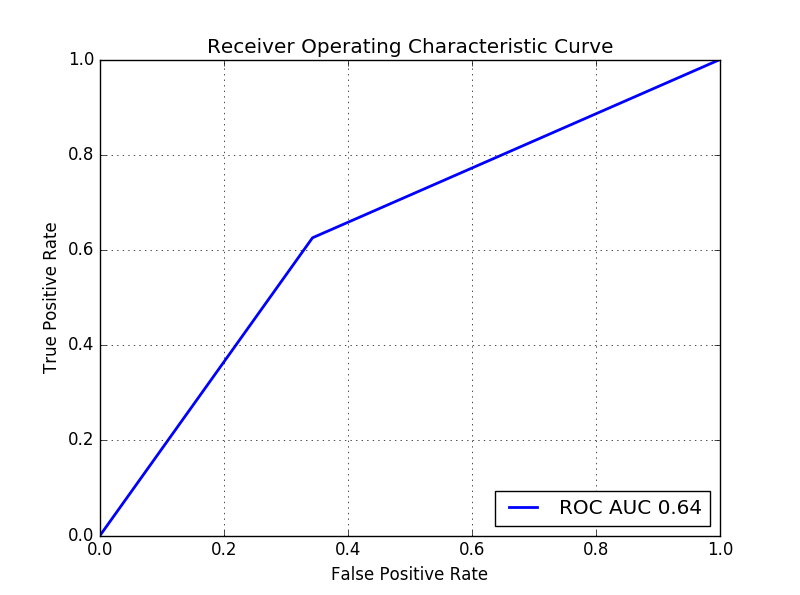
\includegraphics[width=0.9\linewidth]{images/AUC-TestDataset-rbf} 
		\caption{ROC Curve}
		\label{fig:AUC_TestDataset_rbf}
	\end{subfigure}
	\begin{subfigure}{0.5\textwidth}
		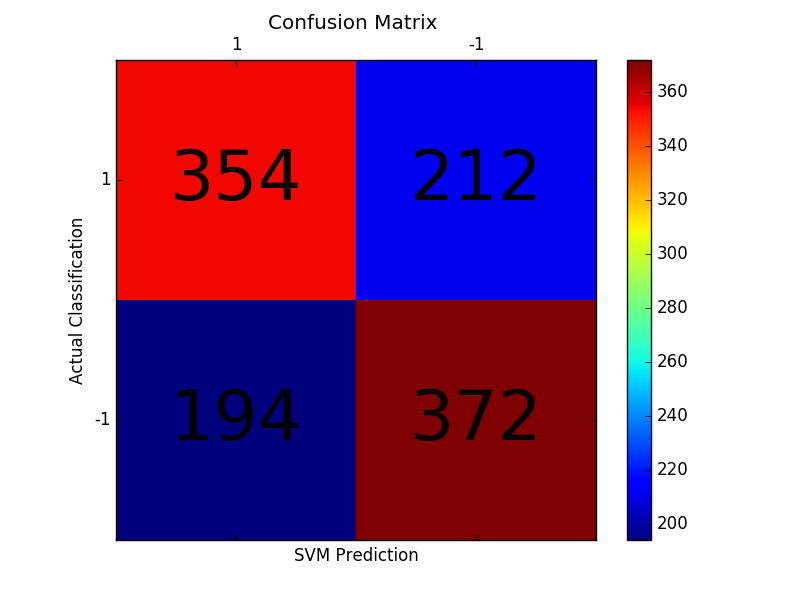
\includegraphics[width=0.9\linewidth]{images/CM-TestDataset-rbf}
		\caption{Confusion Matrix}
		\label{fig:CM_TestDataset_rbf}
	\end{subfigure}
	
	\caption{Test Dataset - RBF Kernel}
	\label{fig:TestDataset_rbf_results}
\end{figure}


\begin{figure}[h]
	
	\begin{subfigure}{0.5\textwidth}
		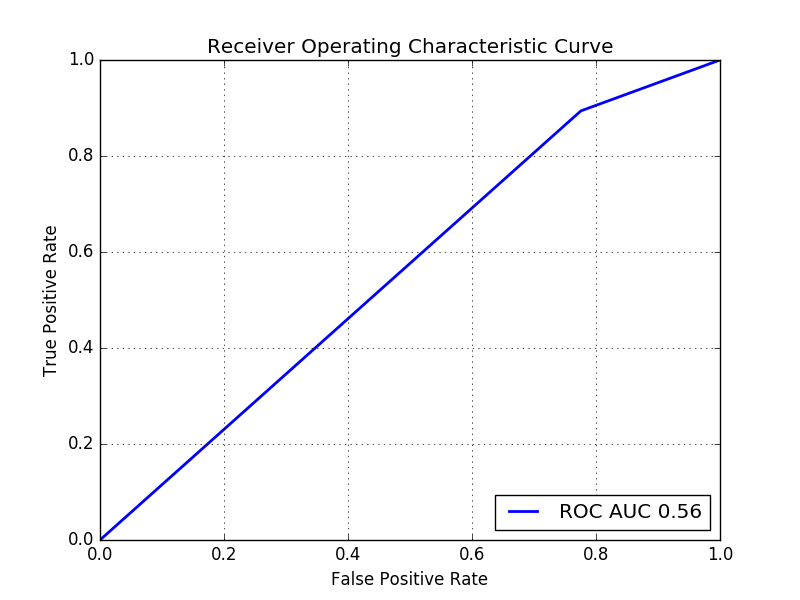
\includegraphics[width=0.9\linewidth]{images/AUC-TestDataset-poly} 
		\caption{ROC Curve}
		\label{fig:AUC_TestDataset_poly}
	\end{subfigure}
	\begin{subfigure}{0.5\textwidth}
		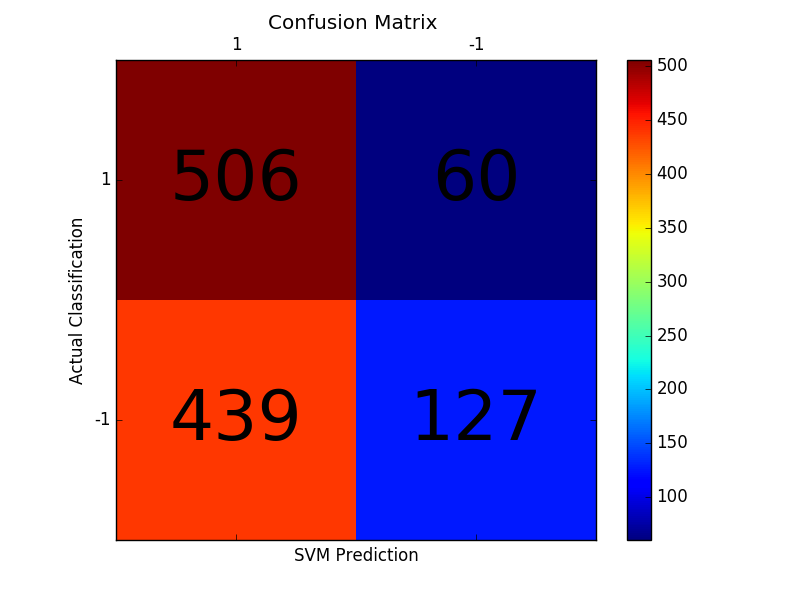
\includegraphics[width=0.9\linewidth]{images/CM-TestDataset-poly}
		\caption{Confusion Matrix}
		\label{fig:CM_TestDataset_poly}
	\end{subfigure}
	
	\caption{Test Dataset - Polynomial Kernel}
	\label{fig:TestDataset_poly_results}
\end{figure}



\section{Feature Selection}



\subsection{Recursive Feature Elimination}

Recursive Feature Elimination (RFE) is a feature selection technique. It is used to get rid of the features that contribute the least to the classification. Here, we use RFE to fine tune the SVM classification for unraveling ham and spam images. RFE assigns weights to features and ranks them according to the amount of contribution towards the classification; and eliminates the least ranked features to enhance the accuracy of SVM.

\subsection{Univariate Feature Selection}
